%auto-ignore
%      this ensures the arxiv doesn't try to start TeXing here.
%!TEX root = super_lattice_models_draft.tex
%      prev line helps TeXShop do the right thing



%%%%%%%%%%%%%%%%%%%%%%%
\section{Super pivotal state sums and tensor networks} \label{state_sums}
%%%%%%%%%%%%%%%%%%%%%%%

\dave{Note to self: look at \cite{beliakova1998} and check for relations.}

In this section we write down a Turaev-Viro-Barrett-Westbury (TVBW) state sum for the super pivotal fusion categories\cite{Turaev1992,Barrett1996}, 
and a tensor network for the ground state wave function of the Hamiltonian constructed in \eqref{ham}.
Very closely related work was presented in~\cite{bhardwaj2016}, 
see also \cite{Bultinck2017, upcoming-paper?}.
We first breifly review the TVBW construction for spherical fusion categories. 
We do so in a way that naturally extends to the super-pivotal case with only minor modifications.
Lastly we use the state sum to write down an explicit wave function for the ground ground state of \eqref{ham}.

%We first give a lightning review of the TVBW state sum construction, via the cut-and-glue formalism.
%Since much is known about TVBW state sums, 
%we present the state sum from a slightly different perspective than usual,
%so that the fermionic version of the state sum can be written in essentially the same way.

We view the state sum as a composition of linear maps from finite dimensional tensor product spaces, starting with with the ``vacuum" $\cc$. 
\kw{Still not convinced that this is a valid way to look at it; maybe I will be convinced when I read further.}
This composition of linear maps can be interpreted as a tensor network, 
which we investigate in the subsequent sections.
Those interested in the details of the original construction are referred to \cite{Turaev1992,Barrett1996}, 
and the one followed here in \cite{Walker2006}. 

%The starting point is a list of data:
%\dave{Is pivotal and spherical the same thing?
%I remember getting quite confused about this in a Muger paper.} %\ethan{I think yes}
%\begin{itemize}
%\item a spherical fusion category $\mcc$,
%\item an oriented 3-manifold $M$,
%\item and a cell decomposition with oriented 1-cells and transversally orientated 2-cells (equivalently, the boundary of the 2-cells has an orientation)
%\end{itemize} 
%from which one defines a partition function $Z(M)$. 

To define these linear maps, we will follow a `cut-and-glue' approach.
Schematically, this proceeds by cutting up the manifold on which we want to evaluate the state sum into many parts. 
We assign vector spaces to each of the cut-up pieces and then 
construct the state sum by gluing these pieces back together with linear maps that are given by performing tensor contractions.
In order for our formalism to be amenable to fermionic modifications, we will need to carry out a 
standardization procedure of the cell decomposition of $M$, in much the same way that we 
performed the standardization procedure to define the lattice Hamiltonian. 
This is the issue to which we first turn. 
Much of the following section is notational; 
readers are invited to familiarize themselves with Figure~\ref{NotationStateSum}
and \eqref{attaching_region}-\eqref{tensor_space}, 
and continue with the next subsection. 



\subsection{Outline of proposed reorganization (KW)}	%%%%%%%%%%%%%%%%%%%%%%%%%%%

\kw{My hope was that the notation and order of presentation below would be in close-to-0final form, but currently
I'm falling short of that goal.}

\kw{Still ion progress.}

Most of this is already in the current draft.

Somewhere in intro to section:  
\begin{itemize}
\item We first review the bosonic TVBW state sum and how to convert it into a tensor network.
We then detail the modifications necessary for the fermionic case.
\item
\end{itemize}

TVBW review subsection:
\begin{itemize}
\item Explain the cell decomp assumptions.
We will work with generic (dual to triangulation) for simplicity, but it's easy to generalize to arbitrary cell decompositions.
\item We will choose auxiliary orientations of the 1- and 2-cells.
The final answer does not depend on these choices.
(Remark somewhere that this version of the state sum is described in Walker2006.)
\item We remark that non-trivial FS indicators makes all of this more complicated.
If all FS indicators were 1, then we could arrange that if $a\in\sob(\mcc)$, then $a^*$ is also in $\sob(\mcc)$.
With non-trivial FS indicators, all we can assume that that $a^*$ is non-canonically isomorphic to some simple object in $\sob(\mcc)$.
\item Explain handle decomposition associated to cell decomp.
\item For each $a,b,c$, we choose a basis $\mcb(a,b,c)$ of $V^{abc}$.
($\mcb(a,b,c)$ is empty if $V^{abc}$ is zero-dimensional.)
Also choose a basis $\mcb^*(c^*, b^*, a^*)$ of $V^{c^*b^*a^*}$ such that the xxx pairing is orthogonal.
(It is sometimes convenient to have the pairing matrix merely diagonal instead of $\delta_{ij}$.)
Define the set $\mcb = \bigcup_{a,b,c} \mcb(a,b,c)$.
For each $\beta\in\mcb$ we denote the dual element of $\mcb^*$ as $\beta^*$.
We define $\Theta(\beta)$ to be the value of the pairing on $\beta$ and $\beta^*$.
\item And, alas, we have to define seven more versions of $\mcb$, corresponding to $V^a_{bc}$, $V_{abc}$, etc.
\item \kw{I now lean toward using the BW(?) trick of choosing a global ordering of the 3-cells, which allows us to choose
1- and 2-cell orientations so that we only need the $V^a_{bc}$ (or $V^{ab}_c$) version of $\mcb$.
Another option is to do it first without the global ordering, then note that we can use the global ordering trick.}
\item We define a labeling of the cell decomposition to be (1) a choice, for each 2-cell $f$, of $a_f\in\sob(\mcc)$, and
(2) a choice, for each 1-cell $e$, of $\beta_e\in\mcb$.
\item Given a labeling of the cell decomposition, we associate a number to each 0-, 1- and 2-cells as follows.
\item To a 2-cell labeled by $a$, we associate $d_a$.
\item To a 1-cell labeled by $\beta\in\mcb(a,b,c)$, and adjacent to 2-cells labeled by $a'$, $b'$ and $c'$,
we associate $\delta_{aa'}\delta_{bb'}\delta_{cc'}\Theta(\beta)^{-1}$.
\item To each 0-cell, evaluation of labeled tetrahedral string net.
(This is zero for incompatible labelings.)
\kw{I think with global ordering trickwe only have one type of tetrahedron}
\item Final define
\be
	\sum_{\text{labelings}} \prod_{\text{3-cells}} D^{-1} \prod_{\text{2-cells}} d_a 
			\prod_{\text{1-cells}} \Theta^{-1} \prod_{\text{0-cells}} \text{Tet} 
\ee
\item \kw{I now lean toward first writing a very general form of the sum (for arbitrary cell decompositions and arbitrary
1- and 2-cell orientations), then regularizing by (1) generic cell decomposition, and (2) 1- and 2-cell orientations
chosen compatible with a global ordering.}
\end{itemize}

Bosonic tensor network section:
\begin{itemize}
\item Goal: rewrite state sum as a tensor network.
\item First observation: the parts coming from 0- and 1-handles are already a tensor network.
A (standard) tetrahedral tensor for each 0-cell, and the vector space $\oplus V^{ab}_c$ at each edge.
\item For the 2-cell factors ($d_a$), we have two options.
Our preferred option is to choose, for each 2-cell, an adjacent 0-cell and then modify the tetrahedral tensor by the 
$d_a$ factor.
(Each 0-cell tensor will have between 0 and 6 such factors, depending on the above choices.)
\item The other option is to make the tensor network larger ...
\item The factors of $D^{-1}$ associated to 3-cells can be handled similarly.
The tensor networks we associate to $Y\times I$ will not have any 3-cells.
\item \kw{I just realized a possible disadvantage of the global ordering trick:
The tensor network associated to $Y\times I$ might have less translation invariance than expected.}
\end{itemize}



%%%%%%%%%%%%%%%%%%%%%%%%%%%%%%
\subsection{Notation, standardization, and Hilbert spaces}
%%%%%%%%%%%%%%%%%%%%%%%%%%%%%%

\kw{Do we need to make it clearer that we are reviewing the bosonic case as a warm-up here?
I was confused on this point.}

In this section we will review the construction of the bosonic state-sum as a warm up, and we 
will do it in a way that readily generalizes to the fermionic setting. 

We start with two pieces of data: 
\begin{itemize}
\item a spherical fusion category $\mcc$, 
\item and an oriented 3-manifold $M$ 
%\kw{I think we should consider changing the to $M$.  We usually use the mathcal letters for categories and plan letters for manifolds.}
%\ethan{agreed, changed.}
possessing a cell decomposition with oriented 2-cells 
%\kw{We should think about whether a plain (non-transverse) orientation would be more convenient}
and oriented 1-cells. 
\end{itemize}
In what follows, we will assume that $M$ is closed for simplicity. We will drop this 
assumption when we discuss wave functions and the shadow world construction. 

Our first order of business is to fatten the cell decomposition into a handle decomposition, 
as was done in Section \ref{standardized_handles}.
Recall that a handle decomposition for a 
3-manifold $M$ is built from a series of $k$-handles, with $k=0,1,2,3$, each of which is identified with $D^k\times D^{3-k}$). 
We will often refer to a $k$-cell and its associated $k$-handle with the same letter. 
We call $S^{k-1} \times D^{3-k}$ the attaching region (or attaching boundary) of the $k$-handle,
and $D^k\times S^{3-k-1}$ the non-attaching boundary.
%The attaching region of a $k$-handle is $S^{k-1} \times D^{3-k}$,
The attaching map of a $k$-handle is a homeomorphism from the attaching region to 
a submanifold of the boundary of the union of the lower-dimensional handles.
The topology of $M$ is encoded by the various attaching maps.
%is built into the attaching regions where different handles are connected, each of which is homeomorphic to $S^k \times D^{n-k}$.
%We are interested in 3-manifolds,
%and hence the attaching regions between between the $(k+1)-$ and $k$-handles are given by
%$S^2 \times D^0$ (3-handles to 2-handles), $S^1 \times D^1$ (2-handles to 1-handles), and $S^{0} \times D^2$ (1-handles to 0-handles).
%%KW k-handles attach to the boundary of the 0, 1, ... k-1 handles, not just the k-1-handles
Although not necessary, we assume the cell decomposition of $M$ is dual to a triangulation for ease of notation.
The standardization procedure is similar to the pitchforkization procedure defined in \eqref{pitchfork_basis} and surrounding text.

%To define the tensors in \eqref{TVBWss} explicitly, 
%it is helpful to standardize each of the cells, 
%and the vector spaces we assign to each cell. 
%Technically, the partition function is built on a handle decomposition, 
%but its useful to label the data associated to each handle by the corresponding cell. 

\begin{figure}
\begin{center}
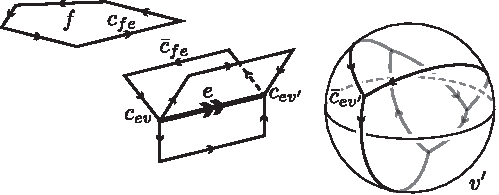
\includegraphics{NotationStateSum.pdf}
\caption{\label{NotationStateSum}
Notation used in this section. 
%The cells can be used to label the weights that determine the partition function.
In the figure we have labeled a 2-cell (face) by $f$, a 1-cell (edge) by $e$, and a 0-cell (vertex) by $v$. 
We assume a cell decomposition that is dual to a triangulation, so that each 1-cell is adjacent to three 2-cells and two 0-cells, 
and each 0-cell is adjacent to four 1-cells. 
The boundary of each 2-cell $f$ possesses an orientation (left). 
The 1-cells are also oriented, with the orientation of the edge $e$ in the figure indicted by the double arrow (center). 
The oriented boundary edge of the face $f$ that neighbors the edge $e$ is labeled $c_{fe}$ (left), 
and the opposing edge that is glued to $c_{fe}$ is labelled by $\bar{c}_{fe}$. 
The trivalent junctions occurring at either end of the edge are denoted $c_{ev}$ and 
$c_{ev'}$ (center).
A small $S^2$ surrounding a 0-cell $v'$ intersects six 2-cells in six oriented lines, which 
meet at four trivalent junctions $\bar{c}_{ev'}$ (right). 
}
\end{center}
\end{figure}

%\ethan{tried (valiantly) to make this more comprehensible, but may have not fully succeeded} 
%\dave{A valiant effort indeed.}


We first establish some notation for the attaching regions of the $k$-handles, which are summarized 
in Figure~\ref{NotationStateSum}. 
We denote the collection of 2-cells by $\mcf$, the collection of 1-cells by $\mce$, and the collection of 0-cells by $\mcv$.
Each $f \in \mcf$ is homeomorphic to a polygon, see `f' in Figure~\ref{NotationStateSum}.
The orientation of $f$ induces an orientation of each edge of the polygon .
%(equivalently, we could say each 2-cell is equipped with a boundary orientation, rather than a transversal orientation).
%Each edge of $f$ is oriented by the orientation assigned to $f$.% (equivalently, each 2-cell is equipped with a boundary orientation).
%We will denote the edge $e$ at the boundary of the 2-cell $f$ by $c_{fe}$.
We will denote the edge at the boundary of the 2-cell labeled $f$ by $c_{fe}$, 
where $e$ is the 1-cell which it attaches to.
(Note the the orientation of the 2-cell and orientation of the 1-cell are chosen independently.)


The 1-handle associated to an edge $e$ intersects three adjacent 2-handles.
%The tubular neighborhood of a given 1-cell $e$ is a 1-handle which intersects three neighboring 2-cells.
% in a collection of three rectangles. %On any given $D^2$ cross-section of 
%a 1-handle, these intersection regions meet at a trivalent vertex. %connected by an annulus with three oriented lines.
The non-attaching boundary of each 1-handle comes equipped with three oriented lines, which match up with 
the edges of the three 2-cells whose boundaries include the 1-cell $e$. For an 
illustration of this, see Figure \ref{One_handle}. 
%The intersections of the three 2-cells with the surface of the 1-handle consists of three lines, 
The orientation of these lines is defined to be opposite to that of the neighboring 2-cell boundaries.
We denote the edge on the boundary of a 1-handle $e$ that matches up with a boundary component 
of the 2-cell $f$ by $\bar{c}_{fe}$, where the bar signifies that the orientation is opposite that of the edge of the 2-cell (see Figure~\ref{NotationStateSum}). 

A 1-cell $e$ connects two 0-cells, $v$ and $v'$. 
A $D^2$ cross-section of the intersection between a 1-handle $e$ and its three neighboring 2-cells 
is a disk with a trivalent vertex in its interior and three marked points on its boundary. 
We will denote the trivalent vertices appearing at either end of $e$ by $c_{ev}$ and $c_{ev'}$.
The orientations of the edges emanating from these vertices are determined by the neighboring 2-cells.
Again, see Figure~\ref{NotationStateSum} for clarification.

A small $S^2$ drawn around a 0-cell intersects six 2-cells and four 1-cells.
For our purposes, it is enough to keep track of the four neighboring 1-cells, 
since they contain all the orientation information that the 2-cells assign to the $S^2$ surrounding the 0-cell.
%Removing a single point from this spherical neighbourhood allows us to define a homeomorphism into the plane. 
%Furthurmore, the gluing regions for the 1-cells can all be taken to be pitchforks as in \eqref{pitchfork_basis}, see Figure~\ref{FIGURE}.
%This is our standardized 0-cell (actually spherical neighbourhood of the 0-cell). 
Denote the 0-cell by $v$ and the neighboring 1-cells by $e_j$, $j=1, \cdots 4$.
Each of the four 1-cells intersects the small $S^2$ at a point where three of the intersections of 
the six 2-cells with the $S^2$ meet. 
We denote these four trivalent junctions by $\bar{c}_{e_j v}$, 
and again the bar denotes that these are in the opposite orientation relative to the trivalent vertices $c_{e_jv}$ at the boundaries of the 1-cells. 

The Figure \ref{NotationStateSum} only shows one representative sample of cells, which all others are homeomorphic to. 
We now standardize each cell so that we can keep track of the topological data associated to the handle decomposition relative to a `standard' one. 
This is analogous to the pitchforkization procedure discussed in the text surrounding \eqref{pitchfork_basis}.
We first note that the spherical neighborhood of an arbitrary 0-cell $v$ can be standardized by removing a point and mapping the resulting picture to the plane. 
We can next `pitchforkize' the attaching region where the four 1-handles are attached to $v$ so that each take the form
\begin{align}
\StandardZeroCell,
\end{align}
or some variant thereof obtained by reversing the orientations of the edges. 
The dashed circles in the above equation are the attaching regions for the 1-handles and again, 
the lines in the above diagram represent the intersections of the six 2-cells 
with the spherical neighbourhood of $v$. 
%whose boundaries include $v$
%with the $S^2$ surrounding $v$. 
The numbers indicate which edge is connected to where on the standard 0-handle, and are associated with $\bar{c}_{e_j v}$.
\kw{I don't understand this last sentence.  What numbers?}

With this standardization procedure, 
the 1-handles which attach two 0-handles are now horseshoe-shaped.
Each 1-handle $e$ can be deformed into the following form:
\begin{align} \label{horshoe_resln} 
\HorshoeIdentity,
\end{align}
where $P_e$ is either the identity, $P$, or $P^2$, where $P$ is the pivot defined in \eqref{Pitchfork_pivot}.
We define $P$ to rotate diagrams counterclockwise relative to the orientation of $e$.
The possible presence of $P$ and $P^2$ is needed to keep track of any relative pivoting
between the pitchforks at either ends of the 1-handles. 


%end of notation bullshit 

%\dave{This sentence has a lot of enthusiasm.} \ethan{:)}
With our vast notational arsenal now fully developed and eager to be utilized, 
we are ready to assign vector spaces to each of the attaching regions $c_{xy}$ defined above.
We define the vector spaces 
\begin{align} \label{EandWdefns}
E = \bigoplus_{x\in\mcc} \cc_x \quad \quad \quad W = \bigoplus_{a,b,c\in\mcc}V^{abc}
\end{align}
where the sums are over a representative set of the simple objects in the input category $\mcc$. 
Momentarily, the vector space $W$ will be assigned to pitchforks.
Not all pitchforks will be oriented with all edges pointing outwards; in this scenario 
we repeat the construction in \eqref{pitchfork_basis} and replace an object labelling an inward-pointing 
edge with its dual. 
The vector space we assign to each of the attachment regions are as follows:
\begin{align}
\label{attaching_region}
  \mch(c_{fe}) &= E \quad \quad \mch(\bar{c}_{fe}) = \mch(c_{fe})^* = E^*\\
\mch(c_{ev} )&= \begin{cases} W &\text{if $e$ is oriented away from $v$} \\
W^* &\text{otherwise} 
\end{cases}\\
\mch(\bar{c}_{ev}) &= \mch(c_{ev})^*
\end{align}
\kw{Shouldn't we have 8 different versions of $W$?}
\dave{There are $8$ versions of it, which we left implicit (see sentences following \eqref{EandWdefns}).
The two referred to in this equation correspond to whether we take our standard basis (if the 1-cell is oriented away from $v$) our the dual basis (the 1-cell is oriented toward $v$).}
The vector space assigned to each $k$-handle is given by tensoring over the vector spaces assigned to each attachment region.
\kw{should say this a little differently; we said above that each k-cell has only one attaching region}
For a 2-handle $f$, a 1-handle $e$, and a 0-handle $v$, we have 
\begin{align}
& \mch(f) = \bigotimes_{c_{ef} \in \partial f} \mch(c_{ef}),  \\
& \mch(e) = \left(\bigotimes_{\bar{c}_{ef} \in \partial e }\mch (\bar{c}_{ef}) \right)\tp \mch(c_{ev}) \tp \mch (c_{ev'}), \\
& \mch(v) = \bigtp_{i=1}^4 \mch(\bar{c}_{e_{i}v}), 
\label{tensor_space}
\end{align}
where as before, $c_{ef} \in \partial f$ are the oriented attachment regions of the 2-cell labeled by $f$, 
and the $\bar{c}_{ef} \in \partial e$ are the lines on the surface of the 1-handle $e$ (the $\bar{c}_{ef}$ are the edges labeled $a,b,c$ in Figure \ref{One_handle}).

From these assignments, we see that if the vector space $V$ is assigned to the region of a $(k+1)$-handle in which it is glued
to a $k$-handle, the corresponding attaching region on the $k$-handle is assigned 
the dual space $V^*$. 
For example, for each $\mch(c_{ev})$ tensor factor in $\mch(e)$, there is a dual tensor factor $\mch(\bar{c}_{ev})=\mch(c_{ev})^*$ in $\mch(v)$.

%\ethan{I think the $e\in f$ and $f\in e$ notation is kinda confusing. Maybe $e\in \partial f$ or something?}
%\dave{I agree, this is tricky.
%Could definitely use some notational insight. 
%It�s doubly confusing since we use the word edge for 3 things at this point. 
%Once for the edges of the 2-cells, once for the corresponding edges on the 1-handles, and again as the thing that we use to identify which 1-handle we are referring to.
%$e \in \partial f$ is great for the 2-cells. 
%But what do we call the edges on the 1-handles ($e in \partial e$ doesn't work.)?
%}
%\ethan{maybe call the 1-handles $t$ (for tube) or something and reserve $e$ for the edges on the 1-handles, so that we can sorta sensibly write $e\in \partial t$ and $e\in \partial f$?}
%The vector spaces have been assigned so that the spaces assigned to the pair of attachment regions on the (k+1)-handle and the k-handle are dual to one another.
%The assignment of vector spaces has been so that the labels of the attachment labels of the (k+1)-handles connecting to the k-handle are dual. 

%\dave{Should this be in the definition section?}
%\ethan{I think keeping it here is good, since we don't use it earlier and in the definition 
%section we aren't pitchforking too hard}%
%\dave{I agree.}

\begin{figure}
\begin{center}
\includegraphics{Onehandle_smaller.pdf}
\caption{\label{One_handle}
Various pictures relating to our presentation of the 1-handles. In the top left picture, we show
three 2-cells which terminate on a given 1-cell, with the orientations of the 2-cells shown. 
In the top right picture we show a 1-handle with its three marked edges and their orientations shown. 
In the bottom left we have the same picture as in the top right, but with the intersection of the 2-cells 
with the 1-handle shaded in color. In the bottom right picture, we show the same picture as in the bottom left, but this time with the vertices standardized via our pitchforkization procedure. 
\dave{Should modify this picture to match text.} \ethan{looks good to me?}
}
\end{center}
\end{figure}



%%%%%%%%%%%%%%%%
\begin{comment}
The fusion category $\mcc$ will allow us to assigns maps from (k+1)-handles to a k-handles via the attaching the attaching maps. 
This is done through the cut-and-glue relation,
\dave{Note to self: Check ch.6 Walker notes.
There's a formula that even looks like the one I want.
It is something like:
}
\begin{align}
Z(M_{\text{gl}}) = \sum_{i,j}Z(M_{\text{cut}} \cup e_i \cup \hat{e}_j)g^{ij}
\end{align}
where $e_i$ and $\hat{e}_j$ are basis of the gluing region on the (k+1)-handle and k-handle respectively, 
and $g^{ij} = (g^{-1})_{ij} $, with $g_{ij} = \langle \hat{e}_j, e_i \rangle_{S^2}$.
This can be simplified by letting $e_i$, and $\hat{e}_j$ run over orthogonal basis for the gluing region and dual gluing region. 
This is done with idempotents etc. 

One can now re-interpret the matrices above $Z(M_{\text{cut}} \cup e_i \cup \hat{e}_j)g^{ij}$ as linear maps from the vector spaces assigned to 
the attaching regions of the (k+1)-handles to the k-handles. 
Abstractly we have,
\begin{align}\nonumber
0 \xrightarrow{??}V(\{ c_3 \}) \xrightarrow{T_{\mcf}} V(\{ c_2 \})  \xrightarrow{T_{\mce}} V(\{ c_1 \})  \xrightarrow{T_{\mcv}} V(\{ c_0 \}) 
\end{align}
where $V(\{c_k \})$ is vector space assigned to the attaching region for the k-handles. 
%\kw{full boundary or non-attaching boundary?}
%\dave{Supposing that non-attaching means what it sounds like, then non-attaching boundary.}
%\kw{more generally, while I think the viewpoint you propose is correct in spirit, when one looks at the details things become a little messier,
%and I doubt it's possible to make a clean (and correct) statement along the lines you propose.}
%\dave{
%I agree it's only worth saying if we can do it cleanly (and obviously has to be correct).
%Lets discuss on Skype.
%The picture I had in mind was to think of each tensor as a linear map from incoming indices, living on (k+1)-handles to outgoing ones living on k-handles.
%Then evaluation of the tensor network is just composition of functions.
%The tensors would be something like basis of net-configurations/local relations on a k-handle sandwiched between
% idempotents on attaching region of $k+1$ handle and idemoptents of outgoing attaching region on $k$ handle.
%}
%Semi-simplicity of $\mcc$ means that each of these vector spaces are finite dimensional.
%Furthurmore, the k-handles are disjoint subsets of $M$ and so the vector spaces appearing above are tensor products of vector spaces associate to each k-handle, e.g., $A(\text{0-handles}) = \tp_{v \in \mcv} A_v$,
%where $\mcv$ denotes the collection of 0-handles, and $A_v$ the vector space assigned to each. 
%The linear maps are naturally described by tensors, 
%and the partition function $Z(M)$ as a tensor trace.
The partition function is given by the image of the composition of the linear maps $T_{\mcv} \circ T_{\mce} \circ T_{\mcf}$, which acts as a projector onto the string-net ground state living at the boundary of $M$. 
%In particular, if $\partial M = \emptyset$, the map $T_{\mcv} \circ T_{\mce} \circ T_{\mcf}$ takes $M$ to a complex number. 
%\begin{align}
%Z(M) \in \text{Im} \; T_{\mcv} \circ T_{\mce} \circ T_{\mcf}
%\end{align}
``Locality" of the handle decomposition means that the linear maps can be expressed as tensor contractions which are local with respect to the handle decomposition.

Denoting the number of 3-cells by $n_3$, the collection of 2-cells by $\mcf$, 
the collection of 1-cells $\mce$, and the collection of 0-cells by $\mcv$, 
the partition function can be written as,
\begin{align}
Z(M) = \frac{1}{\mcd^{2 n_3}}\sum_{\mcl} \prod_{f \in \mcf} T_f \prod_{e \in \mce} T_e \prod_{v \in \mcv} T_v
\label{TVBWss}
\end{align}
where $\mcl$ runs over a label set determined by $\mcc$, 
and the $T_f$, $T_e$, and $T_v$, 
are fixed numbers for a particular labeling. 
Each tensor is solely determined by the labels ascribed to each cell corresponding to the 0-, 1-, and 2-cells,
these numbers are provided by evalutions of diagrams on $S^2$.

Abstractly, the tensors appearing in \eqref{TVBWss}, 
defined by,
\begin{align}\nonumber
\cc \ra A(\text{3-handles}) \ra \tp_{f} A(f) \xrightarrow{T_f} \tp_{e \in \mce} A(e) \xrightarrow{T_e} \tp_{v \in \mcv} A(v) \xrightarrow{T_v} Z(M)
\end{align}
\ethan{note to self: I don't think we've ever defined $A({\rm stuff})$ anywhere. Should find the earliest place we use it and add the defn}
\dave{I changed to $\mch(\text{space})$, 
which I think jibes with what we use earlier.}
where each $T$ is given by,
\dave{Will think about this more carefully in the near term.}
\begin{align}
T = \sum_{\phi, \psi}T_{\phi \psi}  \psi \tp \phi^*
\end{align}
where $\psi$ and $\phi$ are basis vectors in the spaces assigned to $k$-handles and $(k+1)$-handles, respectively. 
For explicit definitions see \cite{Walker2006}.
The above technically gives the correct answer for the fermionic case, 
practical implimentation requires care.
In the next section we present a standardization procedure that allows one to evaluate the partition function.
\end{comment}


%%%%%%%%%%%%%%%%%%%%%%%%%%%%%%%%
\subsection{Constructing the state sum}
%%%%%%%%%%%%%%%%%%%%%%%%%%%%%%%%

We now define the contraction function $\chi$, 
which pairs the vectors in neighboring dual vector spaces and allows us to compute the state sum. 
We define
\begin{align}
\chi: &\mch^* \tp \mch \ra \cc\\
& \mu^* \tp \nu \mapsto \delta_{\mu\nu}.
\end{align}
\kw{Is this the canonical pairing?  If yes, say so; if not, why not?}
This is essentially the same as the bilinear pairing defined in \eqref{reflection_pairing_defn}, just with a different normalization and Koszul ordering on tensor factors. 
It is defined on every pair of tensor factors $\mch(\bar{c}_{xy}) \tp \mch( c_{xy})$
that are assigned 
to attaching regions in the handle decomposition.
On vectors $\mu^* \tp \nu \in (V^{abc})^*\tp V^{abc}$, $\chi$ is proportional to the evaluation of the following `banana' diagram:
\begin{align}
\chi(\mu^* \tp  \nu) \propto \Banana
\end{align}


Since the vector spaces for the attaching regions between $(k+1)-$ and $k$-handles are dual 
to each other, the total Hilbert space 
\begin{align} \label{total_hilb_space}
\mch(M) = \bigotimes_{f \in \mcf} \mch(f) \bigotimes_{e \in \mce} \mch(e) \bigotimes_{v \in \mcv} \mch(v)
\end{align}
admits a decomposition into a subspace tensored with its dual, and hence we have a map
\begin{align}
\label{indicator}
\chi:\; \mch(M) \rightarrow \cc
\end{align}
which is defined on each basis element of $\mch(M)$ and extended to the whole
Hilbert space by linearity.
A state-sum is specified by $\chi(X)$,
where $ X \in \mch(M)$ is a weighted sum of basis vectors, with the 
weights determined by tensors that we will write down shortly. 
%Note that in practice, 
%one has to specify an ordering on all tensor factors in $\mch(M)$, 
%and keep track of the Koszul signs when evaluating the indicator function.
%\ethan{this seems like $X$ is a graph with a particular coloring (since $\chi$ acts on tensor products of particular vectors in the hilbert spaces), but I thought we needed to sum over all (admissible) colorings to get $Z$\dave{It�s defined on each basis element, 
%and extended to the whole vector space by linearity. 
%I guess we should say that.}}

In the case where $\partial M \neq \emptyset$, $\mch(M)$ admits a decomposition as $\mch^*_{bulk} \tp \mch_{bulk} \tp \mch(\partial M)$, where 
the Hilbert spaces of the degrees of freedom on $\partial M$ lack dual tensor factors appearing in $\mch(M)$. 
The partition function is still performed with the help of $\chi$, which contracts out the tensor factors in $\mch^*_{bulk} \tp \mch_{bulk}$ but leaves those in $\mch(\partial M)$ uncontracted, producing a wavefucntion supported on $\mch(\partial M)$ (that is, a map $A(\partial M) \ra \cc$).
\kw{We need to distinguish between $A(Y)$ and $Z(Y)$ here and throughout.
I would say the output is a function from $A(\partial M)$ to $\cc$.}


%\ethan{what follows is commented-out cut-and-glue stuff. Might come back and borrow stuff if we decide to expound on things in that direction}
\begin{comment}
Lastly we define a non-degenerate bilinear pairing between vectors in the vector space assigned to a disk with $n$ marked points. 
It is defined by the evaluation map,
\begin{align}
\mcb:\;  &V^{x_1 x_2 \cdots x_n} \tp V^{x_n^* \cdots x_2^* x_1^*} \ra \cc \\
&\Bilineara \tp \Bilinearb \mapsto \Bilinearc
\end{align} 
where $\mu_i \in V^{x_1 x_2 \cdots x_n}$ and $\nu_j \in V^{x_n^* \cdots x_2^* x_1^*}$. 
This bilinear pairing is just the evaluation map. 
We emphasize that it is $\cc$-linear in both its arguments. 
In particular, it gives us a linear action on each basis element $\mu_i  \in V^{abc}$ for each element  $\nu_j \in V^{ c^*b^* a^*}$. 
The non-degeneracy condition means that the matrix $B_{ij} = \mcb(\mu_i \tp \nu_j)$ is invertible. 
Hence we can define a set of vectors $\mu_j^* = \sum_i \nu_i (B^{-1} )_{ij} $ so that,
\begin{align} 
\mcb( \mu_i \tp \mu_j^*)  = \delta_{ij}
\end{align} 
Note that in most of the paper we have re-scaled these vectors so that 
$B(\mu_i \tp  \mu_j^*) = \sqrt{d_a d_b d_c} \delta_{ij}$ for $\mu_i \in V^{abc}$ and $\mu_j^* \in V^{c^*b^*a^*}$.
\ethan{moved the bilinear pairing thing to the definition section (in the fusion spaces subsection) at Dave's suggestion \dave{I made a comment that maybe we shouldn�t move it here.}}
We will find it helpful to change the normalization of the bilinear pairing \eqref{reflection_pairing_defn} between 
vectors in $V^{x_1\dots x_n}$ and vectors in $V^{x_n^*\dots x_1^*}$.
Namely, in what follows we will work with the normalization 
\be \mcb(\mu_i\tp \mu_j^*) = \delta_{ij}.\ee
\dave{Is the following sensical, or can I just stipulate it.
Also FS indicators? }For the vector space $E$ above, 
it is natural to identify $v_a \in \cc_a$ with $V^{a a^*}_\unit$, and define $\mcb(v_a \tp v_b) = \delta_{ab^*}$.
\dave{What if $a$ is self dual?}
\ethan{then shouldn't it be $\mcb(v_a \tp v_{a^*}) = \kappa_a$?
\dave{I think $\mcb(v_a \tp v_{a^*}) =1$, but $\mcb(v_a\tp v_a) = \kappa_a d_a$. }}
\dave{That's actually a good reason why the above is a bad definition. 
Lets use $\mcb(\mu_i \tp \mu_j^*) = \theta(\mu_i,\mu_j^*) \delta_{ij}$ }

\dave{Kevin, this would be something I'd want you to look at.
}
Lastly we define a `tensor contraction' that will be useful for the state sum.
This is found by extending the bilinear pairing to the tensor product space,
\begin{align}
\mcb: \;\mch(M)  \ra \cc
\label{contract}
\end{align}
where $\mch(M) =  \tp_{f\in \mcf } \mch(f) \tp_{e\in \mce}\mch(e) \tp_{\in \mcv} \mch (v)$. 
This is defined by applying $\mcb$ across all pairs of attaching regions.
For example, 
$$
\mcb: \;  \mch(c_{ef}) \tp \mch(e) \ra \bigtp_{f \notin e}  \mch(\bar{c}_{ef}) \tp \mch(c_{ev}) \tp \mch(c_{ev'})
$$
\dave{Does it make sense?
Do picture example?}
\ethan{I'm a little confused by the notation. Is this map supposed to be contracting out 
a given edge in the 1-handle?}
\dave{Yes.
Maybe its better to just describe in words.
Or replace the $\mch(e)$ in the above with a $ \tp_{f \in e}  \mch(\bar{c}_{ef}) \tp \mch(c_{ev}) \tp \mch(c_{ev�})$}
\dave{This also highlights how awful the $f \in e$ notation is. 
Lets think of something better.}
\ethan{so then should it actually be $\bigtp_{f'\in e, f'\neq f}$ on the RHS?}
\dave{This is basically a PEPS.}
\dave{To Dave:
Cite Levin's tensor trace paper?
I think they essentially did the same construction, but will need to check.}
\end{comment}



We can now write down the Turaev-Viro-Barrett-Westbury state sum in the language and notation discussed above.
The benefit of defining \eqref{indicator} is that we can now define a partition function by specifying a vector in $\mch(M)$ to evaluate with $\chi$.
Since the construction for the bosonic state sum is well known (see the original works \cite{Turaev1992,Barrett1996}), 
we will just provide the answer and then move on to the fermionic version of the state sum. 

%We now specify three sets of tensors $T_f$, $T_e$, and $T_v$, living the in vector spaces defined in \eqref{tensor_space}. 
%Correspondingly, 
%we define a set of tensors 
As said above, the partition function is defined by writing down a set of tensors for each 2-handle $f$, 1-handle $e$, and 0-handle $v$:
\begin{align}
T_f &= \sum_{w_f \in \mch(f)} T_f(w_f) w_f, \\
 T_e &= \sum_{w_e \in \mch(e)} T_e(w_e) w_e, \\
  T_v &= \sum_{w_v \in \mch(v) } T_v(w_v) w_v,
\end{align}
where each sum runs over the orthogonal basis vectors of the indicated Hilbert space, 
and the tensor is defined by assigning a particular weight to each basis vector. 
The partition function is given by the tensor contraction
\begin{align}
Z(M)  = \chi \left( \bigotimes_{f \in \mcf}  T_f \bigotimes_{e \in \mce}  T_e \bigotimes_{v \in \mcv}  T_v \right). 
\label{ZTensor}
\end{align}
Using linearity, this can be written in more conventional notation as  
\begin{align}
Z(M) = \sum_{\{ w_f \} } \sum_{\{ w_e\}} \sum_{\{ w_v \}} \prod_{f \in \mcf} T_f(w_f) 
\prod_{e \in \mce} T_e(w_e) \prod_{v \in \mcv} T_v(w_v) 
%\chi \left(\bigotimes_{f \in \mcf}  w_f \bigotimes_{e \in \mce}  w_e \bigotimes_{v \in \mcv}  w_v \right) 
\chi(w_\mcl)
\end{align}
where the sums are over all possible basis vectors of $\mch(f)$, $\mch(e)$, and $\mch(v)$, and
where we have defined 
%where the sums are over all possible string-net colorings of the faces, edges, and vertices, and
%where we have defined 
\be w_\mcl = \bigotimes_{f \in \mcf}  w_f \bigotimes_{e \in \mce}  w_e \bigotimes_{v \in \mcv}  w_v\ee
for a particular 
choice of
% string-net colorings 
$w_f,w_e,$ and $w_v$.
%We will call a labeling $\mcl$ of the cell decomposition {\it admissible} if $\chi(w_\mcl) =1$.
%The state sum can then be written as
%\begin{align} 
%Z(M) = \sum_{ \mcl } \prod_{f \in \mcf} T_f(w_f) 
%\prod_{e \in \mce} T_e(w_e) \prod_{v \in \mcv} T_v(w_v), 
%\label{ZConventional}
%\end{align} 
%where the sum over labelings $\mcl$ is restricted to run only over all admissible labelings $\mcl$. 
%\kw{Do we really need to introduce admissible labelings?}
%\ethan{no, don't think so. Commented out}
This is the familiar form of the partition function given in \cite{Turaev1992,Barrett1996}.

Now we need to define the tensor weights appearing in our expression for the partition function.
For a 2-cell $f$ with $r$ edges, the 2-cell tensor $T_f(w_f)$ is given by
\begin{align} 
T_f(w_f) = T_f(w_{a_1} \tp w_{a_2} \tp \cdots \tp  w_{a_r})   =\sum_{v_x^* \in E} d_x \prod_{i = 1}^r \chi(v_x^* \tp w_{a_i})
% \sum_{x, \; \{ v_{a_{e}}\} \;  : \;e \in f} \left( d_x  \prod_{e \in f} \delta_{x, a_e} \right)   \bigtp_{e \in f}v_{a_e}
\end{align} 
%\begin{align}
%T_f(\tp_{e \in f} a_e) = \sum_x d_x \prod_{e \in f}  \delta_{x, a_e}
%\end{align}
%where each $a_e$ is a basis vector of $A(c_{fe})$.
%\dave{Should we we also draw pictures for each tensor?
%usually good practice for string nets to do (labeled picture) = number}
%For example, for a pentagonal 2-cell we can diagrammatically denote the matrix elements of this tensor as
%\begin{align}
%\FaceWeight = \sum_{x} d_x \prod_i \delta_{x, a_i}
%\end{align}
Note that this tensor is only non-zero if all edge labels of the boundary 1-cells of the 2-cell $f$ are the same.


Now consider a 1-cell $e$. 
Suppose that the boundary 0-cells at the ends of $e$ are labeled as $v$ and $v'$, with $e$ oriented from $v$ to $v'$. 
Let $w_e = v_{a_1} \tp v_{a_2} \tp v_{a_3} \tp \mu \tp \nu$, with $v_{a_i}$ basis vectors in $\mch(\bar{c}_{ef_i})$ for each 2-cell $f_i$ neighboring $e$, and $\mu,\nu$ 
basis vectors in $\mch(c_{ev})$ and $\mch(c_{ev'})$, respectively. We then have
\begin{align}
T_e(w_e) = T_e(v_{a_1} \tp v_{a_2} \tp v_{a_3} \tp \mu \tp \nu^*) = \frac{\mcb(\mu \tp P_e(\nu_j^*))}{\mcb(\mu \tp \mu^*) \mcb(\nu \tp \nu^*)},
\end{align}
where $\mcb$ is the pairing defined in \eqref{b_pairing_defn} (which differs from $\chi$ only in its normalization). 
As before, $P_e$ encodes the pivot of the 1-handle $e$ (i.e.\ to what degree the pitchforks at either 
end of $e$ differ by $2\pi/3$ rotations).%, and $P_e(\nu_j)$ is zero unless $\text{id}_{a_{1^* }\tp a_{2^*} \tp a_{3^*}} \circ \nu_j = \nu_j$.
Since each 1-handle has three edges, there are $2^3 = 8$ possible orientations that the edges of a given 1-handle can have, 
and hence there are technically $8$ different 1-cell tensors to specify, differing by the presence of either vectors or their duals in the expression for $T_e$ above. 
\dave{Sphericity halves this number.}

Lastly we define the 0-cell tensors $T_v$, which map vectors in $\mch(v)$ to complex numbers. 
The matrix elements of the $T_v$ tensors are defined as evaluations of tetrahedral string-nets whose vertices have been transformed into the pitchfork convention.
That is, 
\begin{align}
T_v(\alpha \tp \beta \tp \gamma \tp \delta) = \Tetrahedron
\end{align}
%where the tetrahedral symbol is defined in our standardization convention by 
%\begin{align}
%\text{Tet}(\alpha \tp \beta \tp \gamma \tp \delta) =\; \Tetrahedron
%\label{Tetrahedron}
%\end{align}
We have defined the tensor by its evaluation on the right with 
$\alpha \in \bigoplus_{abc} V^{abc}$, $\beta \in \bigoplus_{a^* bc} V^{a^* bc}$, $\gamma \in \bigoplus_{a^* b c^*} V^{a^* b c^*}$, and $ \delta \in \bigoplus_{a^* b^* c^*} V^{a^* b^* c^*}$.
We have defined this tensor for a particular collection of edge orientations, but generically %; one can flip the direction of an arrow by taking the appropriate object label to its dual. 
there are $2^6 = 64$ possible collections of edge orientations, each of which requires its own $T_v$ tensor and is given by the appropriate diagram evaluation with $\alpha,\beta,\gamma,\delta$ chosen from the appropriate fusion spaces 
\footnote{Not all these $64$ tetrahedra are independent however, as 
some of them can be transformed into one another by using the pivotal and spherical structure of the input category.}. 

Plugging the tensors into \eqref{ZTensor} (or equivalently into \eqref{ZConventional}), one finds the explicit presentation of the TVBW state sum in terms of the evaluation of string-net pictures. 


%Finally, we can write down the TVBW state sum as
%\begin{align}
%Z(M) = \mcb(\tp_{f \in \mcf} T_f \tp_{e \in \mce} T_e \tp_{v \in \mcv} T_v)
%\end{align} 
%where $\mcb$ is used in the sense of \eqref{contract}.
%Lastly we would like to comment that this is the same as the state sum, 
%where one sums over all possible compatible labelings of the attaching regions, with the appropriate weights defined by the tensors above. 
%The benefit of writing the partition function this way 
%is that we can write down the state sum in the fermionic case with little modification. 

%The 1-cell weights are given by $T_e \in A(e)^*$ defined via,%
%\begin{align}
% T_e(\mu_v \tp a_{1}^*\tp a_{2}^* \tp a_{3}^* \tp \mu_{v'})  = 
% \begin{cases} 
 %\phi(\mu_v, \mu_{v'})^{-1}  & \text{if labels agree} \\
% 0 & \text{otherwise}
% \end{cases} 
%\end{align}%
%where $\phi(*,*)$ is the pairing between a disk and a reflected disk. 
%Or diagrammartically we write this as,
%\begin{align}
%\EdgeTensorprime = 
 %\begin{cases} 
% \phi(\mu_v, \mu_{v'})^{-1}  & \text{if labels agree} \\
% 0 & \text{otherwise}
 %\end{cases} 
%\end{align}
%Note that for this to be non-zero $\mu_v \in V^{a_1^* a_2 a_3}$ and $\mu_{v'} = \mu_{v}^*$.
%\dave{What if $a \cong a^*$?}




%\begin{figure}
%\begin{center}
%
\includegraphics{HorshoeTube.pdf}
%\caption{\label{HorshoeTube}
%\dave{Will use this later.}
%}
%\end{center}
%\end{figure}



%%%%%%%%%%%%%%%%%%%%%%
\subsection{The fermionic state sum}
%%%%%%%%%%%%%%%%%%%%%%

The fermionic version of the state sum can be computed using the technique described above.  
Here we present only the result, since the methods involved are exactly the same as in the bosonic case.

As in the bosonic case, there are two pieces of input data for the state sum, 
which each acquire extra adjectives in the fermionic setting:
\begin{itemize}
\item a super pivotal fusion category $\mcc$,
\item and an oriented spin 3-manifold $M$ possessing a cell decomposition with orientations of 1- and 2-cells.
\end{itemize}
We will employ the same notation used in the previous section. 
The vector spaces $E$ and $W$ which are assigned to the attaching regions are again defined in the same way. 
Note however, that $W$ is a super vector space, while $E$ remains bosonic
\footnote{A natural choice for the edge vector space is $E'=\oplus_x\End(x)$, which is generically a 
super vector space, with odd vectors corresponding to q-type edges which host fermionic dots. However, one 
can always use odd endomorphisms and the fact that each 2-cell inherits a bounding spin structure to displace these odd degrees of freedom to the vertex Hilbert spaces. This procedure results in a simpler (purely bosonic) edge Hilbert space $E$. 
\kw{I disagree that $E'$ is a natural choice.
I think there is some misunderstanding here about how the TQFT gluing rules are being used.
This is problem elsewhere in this section too -- not just this footnote.}
%\dave{What's the benefit? Or are you just saying that there is none?
%Also these vector spaces don't have vertices associated with them.}
%\ethan{I'm saying that I think the natural edge Hilbert space is $E'$, which is super, as opposed to $E$, which isn't. We can still use $E$, but I wanted to explain why.}
%\dave{Where are the vertices that you're displacing the fermions?
%On the 1-cells?}
%\ethan{On the ends of the 1-cells. So for the 1-handle Hilbert space we have $\mch(e) = E^{\tp 3} \tp %W \tp W^*$, and we can take the fermionicness of the $E$ factors and displace it onto the $W$ factors, leaving the $E$s bosonic.}
%\dave{Ok. But the 2-cells don't have this option.}
}.
%\ethan{You said $E$ was bosonic, but I was initially thinking that $E = \oplus_x \End(x)$?}
%\dave{We could write it as $(\text{End}(x))^0$ if we want. 
%But I think we should keep them bosonic.}
%In the fermionic case the vector space $W$ is a super vector space, while $E$ remain a purely bosonic (even) vector space. 

There are three main differences present in the construction of the fermionic state sum. 
Although we have largely been using unordered tensor products throughout our discussion of fermionic theories, to actually compute
the partition function through a tensor contraction, a particular choice of ordering for the tensors involved in the partition function must be made (with different orderings related by the usual Koszul signs).
%\dave{Need to say ordering on what.
%I would be inclined to say that we need an ordering for every tensor. 
%And then give a prescription to contract over tensors and find a possibly large tensor, with another ordering.}
Secondly, since simple objects in $\mcc$ can have non-trivial endomorphism algebras, some additional care must be taken to ensure the proper normalization of the partition function. 
Finally, spin structure considerations means that the pivot $P_e$ appearing in the definition of the fermionic 1-cell tensor $T_e$ has different properties 
than the one appearing in the bosonic partition function. 


%Except now one must of course define a sign ordering in the tensor product.
%We again define the contraction in \eqref{contract}.
%This is defined on the un-ordered tensor product defined in \ref{koszul_signs}.
%To get a number at the end of the day, one still has to choose a definite ordering of the tensor product spaces, and
%when applying $\mcb$, one needs to have the correct order of tensor factors.
%We will continue to adopt the implicit notation where the Koszul ordering increases
%from left to right in tensor factors. 
%Mapping an arbitrary Koszul ordering to this standard ordering can always be done with a finite number of Koszul isormorphisms.
%\dave{Check Turzillo paper.}
%\dave{I found that the $\mcb(\psi_1 \tp \eta_2) = \mcb(\eta_1 \tp \psi _2)$ is symmetric. }

The difference in the allowed endomorphism algebras for the simple objects in $\mcc$ leads to a modification of 
the 2-cell tensors, which is needed to account for the fact that $\dim\End(x)\neq1$ if $x$ is q-type.
The fermionic version of the 2-cell tensor at a face $f$ with $r$ boundary edges is 
\begin{align}
T_f(w_f)=T_f(w_{a_1} \tp w_{a_2} \tp \cdots \tp  w_{a_r})   =\sum_{v_x^* \in E} \frac{d_x}{\text{dim} \; \text{End}(x)}
\prod_{i = 1}^r \chi(v_x^* \tp w_{a_i}).
\end{align}
This is the same $\text{dim} \; \text{End}(x)$ that appears in the definition of the total quantum dimension $\mcd$ (see \ref{total_qdim_defn}). 
%\dave{removed the following for now.}
%Since the 2-cells inherit a bounding spin structure, any closed loop of string embedded in the 2-cell will 
%have even fermion parity, and so the vector space for the 2-cell tensors remains bosonic, and as such needs no further adjustments for the fermionic setting. 
%\ethan{right?}
%\dave{The tensors always have even parity. \ethan{because of what I wrote above, right?}
%The normalization is because it's the trivial idempotent that we plug into the $S^1 \times D^1$ attaching region in the cut and glue picture. \ethan{agreed}
%}

The contraction map $\chi : \mch^* \tp \mch \ra \cc$ serves the same purpose as in the bosonic case, 
but in the fermionic setting we must be careful to address Koszul ordering issues correctly. 
We will define $\chi$ to act on two tensors with {\it adjacent} Koszul ordering. That is, in order
to contract $w^*\tp v$ using $\chi$, the Koszul ordering of $w$ and $v$ must be $w^*_i \tp v_{i+1}$ for some $i\in \zz$. If we are 
instead given $w_i^*\tp v_j$ for $j\neq i+1$, in order to evaluate $\chi(w^*\tp v)$ we must permute the Koszul ordering so that $j\mapsto i+1$, at the cost of the usual Koszul signs. 
\ethan{strictly speaking, I don't think we need the following (it could just confuse people)}
Under re-arrangement of tensor factors and Koszul signs, $\chi$ behaves as
\begin{align}
\delta_{wv} = \chi(w^* \tp v)=(-1)^{|v| |w|} \chi(w^*_2 \tp v_1) = (-1)^{|w|}(-1)^{|v| |w|} \chi(v \tp w^*) = (-1)^{|w|(|v|+1)} \delta_{v^* w^{*}},
\end{align}
%\dave{This difference in ordering may Koszul headaches later.}
%\ethan{Don't we usually have $\mch^*\cong\mch$ so that the difference is just a matter of labeling? %However, might be best to dualize the definition of $\chi$}.
%\dave{What does it mean to dualize the definition of $\chi$?}
where as usual, the numerical subscripts indicate an explicit Koszul ordering, and the absence of subscripts 
indicates the standard ordering convention, which increases from left to right. 
The sign $(-1)^{|w|}$ appears 
when performing a $2\pi$ rotation $P^3 = (-1)^F$ on the vector $w$ when interchanging the order of the tensor factors (recall that graphically, $a\tp b$ corresponds to placing $a$ and $b$ side-by-side horizontally).
Since $\chi(w^*\tp v)$ is nonzero only when $w$ and $v$ have the same parity, this reads $\chi(w^*\tp v) = \chi(v\tp w^*)$. 


The tensors for the one-handles are also modified when passing to the fermionic setting. 
In the bosonic state sum, we needed to keep track of three possible pivots
in the resolution \eqref{horshoe_resln}.
For the fermionic state sum $P^3 = (-1)^F$, meaning that $P_e$ now has order 6 and we now have six possible pivots:
in addition to the three we could have in the bosonic state sum (id, $P$, and $P^2$), 
we can also have an action of the spin-flip $P^3$; recall \eqref{spin_flip_functor}.
The pivots carry spin structure data, with the product of all pivots over a closed path 
determining the fermionic boundary conditions along that path. The $P_e$ terms 
play a similar role to the $\alpha(e)$ variables employed in our construction 
of the lattice Hamiltonian in Sec. \ref{standardized_handles}. 
With the appropriate generalization of the $P_e$ operators to the fermionic case, 
the edge tensors retain the same form as in the bosonic state-sum, namely
\begin{align}
T_e(v_{a_1} \tp v_{a_2} \tp v_{a_3} \tp \mu \tp \nu^*) = \frac{\mcb(\mu \tp P_e(\nu^*))}{\mcb(\mu \tp \mu^*) \mcb(\nu^* \tp \nu)} ,
%T_e = \sum_{i,j, \; \{ v_{a_r}\} \; :\; r \in e} \mcb(\mu_i \tp P_e \circ \nu_j^*) \tp_{r \in e} v_{a_r}^* \tp \mu_i \tp \nu_j^*
\end{align}
except for the fact that $P_e$ now has order 6, with $P_e^3=(-1)^F$. 
\dave{Need to check ordering on this.}
%\dave{are equivalence classes of spin structures in 1-1 with $\{ P_e \}$? 
%May be worth commenting on, it seems unlikely that this is the case.
%}
As before, we assume that 
the edge $e$ ends on the 0-cells $v,v'$, is oriented from $v$ to $v'$, and that 
$\mu$ is a basis vector in the Hilbert space $\mch(c_{ev})$ and $\nu$ is a basis vector 
in $\mch(c_{ev'})$.
%Additionally, we need to keep track of the Koszul ordering in above the tensor product. 
%In the above we assumed the standard implicit left-to-right ordering convention. 
%If we are given an ordering that departs from this convention, 
%we must introduce the appropriate Koszul sign required to standardize the order. 
%\dave{Which ordering are you referring to? 
%It seems like it's already fixed in the above.}

The 0-cell tensors are exactly the same as in the bosonic case, 
except that we must keep track of an ordering of the four tensor factors when defining the tetrahedral symbol. 
We choose the following ordering convention:
\begin{align}
T_v(w_v)=T_v(\alpha \tp \beta \tp \gamma \tp \delta) = \Tetrahedron.
% = \sum_{\mu_{e_j} \in \mch(\bar{c}_{e_j v}) } \text{Tet}(\mu_{e_1} \tp \mu_{e_2} \tp \mu_{e_3} \tp \mu_{e_4} )  \mu_{e_1} \tp \mu_{e_2} \tp \mu_{e_3}\tp \mu_{e_4}
\end{align}
%with
%\begin{align}
%\text{Tet}(\alpha \tp \beta \tp \gamma \tp \delta) =\; \Tetrahedron.
%\label{Tetrahedron}
%\end{align}
%If we are given a tetrahedron with a different ordering, we must change the ordering to the standard one, which as usual is done at the cost of the appropriate Koszul signs. 
%\dave{I thought by assumption the 1-cells meeting a tetrahedron are ordered?}
%\dave{I think the only Koszul signs we have to worry about are those appearing in the tensor contraction.}
As an example, in the $C_2$ theory there are 32 non-zero $T_v$ tensor weights to specify. If we write $V^{\unit\unit\unit} = \langle1\rangle,V^{\beta\beta\unit}=\langle v_e,v_o\rangle$ with $v_o$ odd, 
then a few examples of $T_v$ tensor weights are $T_v(v_o\tp v_o\tp 1\tp v_e) = T_v(v_o\tp 1\tp v_e \tp v_o) = A^4d$ and 
$T_v(v_o\tp v_e\tp 1 \tp v_o) = T_v(v_o\tp v_e \tp v_o \tp 1) = -d$\footnote{In evaluating these, we have used 
the convention in which a fermionic dot at a vertex $v$ is displaced onto the right-most 
$\beta$ string terminating at $v$.}. \ethan{this is just a reminder
to write down some examples if we feel the need to be a little more friendly / verbose}

The fermionic partition function can be written formally in the same way as before:
\begin{align} \label{simple_fermion_Z}
Z(M) = \chi\left( \bigotimes_{f \in \mcf} T_f \bigotimes_{e \in \mce} T_e \bigotimes_{v \in \mcv} T_v\right),
\end{align}
%where the fact that the tensors are all even means that the order on the tensor product does not matter. 
However, when evaluating the RHS, 
one has to be careful about Koszul sign issues when performing the tensor contraction induced by $\chi$. 
In the above equation, the Koszul ordering of each tensor factor is determined in the usual implicit way, 
so that it increases from left to right on the page. However, this ordering will almost always not be 
the ordering required to provide a valid input for the contraction map $\chi$.
Re-arranging the Koszul ordering given by the left-to-right convention produces a Koszul sign not
present in the bosonic partition function. 

We will now elaborate on the above comments. 
When we contract out two tensor indices of a tensor in $\mch^*\tp\mch$ with $\chi$, we must be careful to only perform 
the contraction on two tensor factors that have adjacent Koszul ordering in the tensor product. 
For example, suppose we have two tensors $Q \in V_Q$ and $T\in V_T$,
defined by
\begin{align}
Q &= \sum_{q_L \tp q \tp q_r } Q(q_L \tp q \tp q_R)q_L \tp q \tp q_R,\\
T &= \sum_{t_L \tp t \tp t_R} T(t_L \tp t \tp t_R  )t_L \tp t \tp t_R,
\end{align}
where we have split the vector spaces $V_Q$ and $V_T$ into tensor factors on 
the left and right of the two indices that we would like to contract, namely $t \in V$ and $q \in V^*$.
We define the contracted tensor by $K$, which is given by
\begin{align}
K = \sum_{ q_L \tp q_R \tp t_L \tp t_R}K(q_L \tp q_R \tp t_L \tp t_R) q_L \tp q_R \tp t_L \tp t_R,
\end{align} 
with 
\begin{align}
\label{contraction_example}
K(q_L \tp q_R \tp t_L \tp t_R) &= \sum_{q,t} Q(q_L \tp q \tp q_R)R(t_L \tp t \tp t_R  ) (-1)^{|q| |q_r|}(-1)^{|t_L| | t|} \chi(q \tp t)\\
&= \sum_{t} Q(q_L \tp t^* \tp q_R)R(t_L \tp t \tp t_R  ) (-1)^{|t|( |q_R| +|t_L|)}.
\end{align}
In the above, we have used the fact that $\chi$ is an even map, meaning that $\chi(q\tp t)$ is only non-zero
if $|q|=|t|$. 
The Koszul sign $(-1)^{|t|( |q_R| +|t_L|)}$ is picked up from commuting the tensor factors $q$ and $t$ next to one another, so that they have the correct Koszul ordering for being input into the contraction map. 

In the above examples, we have used the implicit left-to-right Koszul ordering convention.
In practice, we will more often be performing a contraction on a series of tensors whose Koszul
orderings are indicated explicitly by numerical subscripts, since this notation is better suited to 
our diagrammatic formalism. For example, we have 
\be Q\tp T = \sum_{q_L \tp q \tp q_r } Q(q_L \tp q \tp q_R)T(t_L \tp t \tp t_R  ) q_{L1} \tp q_2 \tp q_{R3} \tp t_{L4} \tp t_5 \tp t_{R6}.\ee
We would like to contract out the indices $t\in V,q\in V^*$, but in order to do this they must have adjacent Koszul ordering. 
To obtain such an 
order, we use the following manipulations:
\begin{align} q_2 \tp q_{R3} \tp t_{L4} \tp t_5 & = (-1)^{|q||q_R|}q_3 \tp q_{R2} \tp t_{L4} \tp t_5 \\ & = (-1)^{|q||q_R|+|t||t_L|} q_3 \tp q_{R2} \tp t_{L5} \tp t_4.
\end{align}
We are now ready to contract out the $q$ and $t$ indicies. The Koszul sign we pick up, namely 
$(-1)^{|q||q_R|+|t||t_L|}$, is of course the same as the one obtained with the implicit left-to-right Koszul ordering convention. 


%For example, suppose we have two tensors $X \in V_1 \tp \dots \tp V_n$ and $Y \in W_1\tp \dots \tp W_m$,
%defined by
%\begin{align}
%X = \sum_{x_i \in V_i}X(x_1 \tp x_2 \tp \cdots \tp x_n) x_1 \tp \cdots \tp x_n,\\
%Y = \sum_{y_i \in W_i}Y(y_1 \tp y_2 \tp \cdots \tp  y_m) y_1 \tp \cdots \tp y_m,
%\end{align} 
%and suppose we want to contract over the indices $x_p$ and $y_q$ in the tensor $X\tp Y$, where $V_p \cong W_q^*$.
%If we denote the contracted tensor by $Z$,
%then 
%\begin{align}
%Z = \sum_{\substack{x_i \in V_i, i \neq p\\ y_j \in W_j, j \neq q}} Z(x_1 \tp \cdots \tp x_{p-1} \tp x_{p+1} \tp \cdots \tp x_n \tp y_1 \tp \cdots\tp y_{q-1} \tp y_{q+1} \tp \cdots \tp y_m) \\
%\times x_1 \tp \cdots \tp x_{p-1} \tp x_{p+1} \tp \cdots \tp x_n \tp y_1 \tp \cdots\tp y_{q-1} \tp y_{q+1} \tp \cdots \tp y_m
%\end{align}
%where 
%\begin{align} \label{contraction_example}
%Z(x_1 \tp \cdots \tp x_{p-1} \tp & x_{p+1} \tp \cdots \tp x_n \tp y_1 \tp \cdots\tp y_{q-1} \tp y_{q+1} \tp \cdots \tp y_m) \\ 
%=& \sum_{x_p \in V_p, y_q \in W_q}X(x_1 \tp \cdots \tp x_n)Y(y_1 \tp\cdots \tp  y_m) \\ & \qquad \times (-1)^{|x_p|(|x_{p+1}| + \cdots + |x_n|)} (-1)^{(|y_1| + \cdots + |y_{q-1}| ) |y_q|} \chi(x_p \tp y_q).
%\end{align}
%The Koszul signs appearing in the above equation are simply those acquired when re-ordering the tensor factors in $X \tp Y$ so that $x_p$ and $y_q$ appear in the order $x_p\tp y_q$, with no other 
%intervening tensor factors. 

The Koszul signs that appear in this example arise when performing the tensor contraction induced by $\chi$ in the 
partition function \eqref{simple_fermion_Z}.
To be slightly more explicit, we can write 
\begin{align} 
Z(M) = \sum_{ \mcl } (-1)^{k_\mcl} \prod_{f \in \mcf} T_f(w_f) 
\prod_{e \in \mce} T_e(w_e) \prod_{v \in \mcv} T_v(w_v),
\end{align} 
where $\mcl$ runs over all admissible labels and $(-1)^{k_\mcl} = \chi(w_\mcl)$ is the Koszul sign acquired 
when re-arranging the Koszul ordering of the tensor factors in $w_\mcl$ when performing the tensor contraction. 
When we form the total Hilbert space The Koszul sign can be found 
by ensuring that tensor factors 
being contracted always have adjacent Koszul-ordering and by using \eqref{contraction_example} repeatedly.


\begin{comment} 

%%%%
%%%%
%%%%
\dave{A sketch of the alternative we discussed on Skype.}
\ethan{I kinda liked having the $T$s be tensors, but I guess no strong preference}
\begin{align}
Z(M)  = \sum_{\mcl} (-1)^{\mcl}\prod_f T_f \prod_e T_e \prod_v T_v
\end{align}
where $\mcl$ runs over all labelings of the tetrahedra. 
An admissible labeling is one a basis vector of the 0-cells defined \eqref{tensor_space}.
A labeling all the 0-cells determines a labeling of all the 1-cells and 0-cells, see Figure \ref{NotationStateSum}.
All we need to do is define the appropriate weights for each cell. 

The zero cell weights are,
\begin{align}
T_v =\text{Tet}(\mu_{e_1} \tp \mu_{e_2} \tp \mu_{e_3} \tp \mu_{e_4} ) 
\end{align}
where the tetrahedral symbol is defined by 
\begin{align}
\text{Tet}(\alpha \tp \beta \tp \gamma \tp \delta) =\; \Tetrahedron
\label{Tetrahedron}
\end{align}

The 1-cell, $e$ oriented from $v$ to $v^\prime$ labeled $\mu_v$ and $\nu_{v^{\prime} }^*$, and edge pivot $P_e$ has weight,
\begin{align}
T_e(\mu_v \tp \nu_{v^{\prime} }) = \frac{\mcb(\mu_v^* \tp P_e(\nu_{v^\prime}) )}{\mcb(\mu_v^* \tp \mu_{v}) \mcb(\nu_{v�} \tp \nu_{v^\prime}^*)}
\end{align}
where $\mcb$ is the bilinear pairing (not kronnecker delta).
\dave{I think I was consistent with $*$ in this equation, but may have flipped every one.}

The 2-cells get a factor of $d_x$. 

Fermionic modifications. 
Again sum over all possible label sets. 
For each labeling define an ordering on all odd pitchforks (or define a global ordering). 
Define,
\begin{align}
Z(M)  = \sum_{\mcl} (-1)^{k_\mcl}\prod_f T_f \prod_e T_e \prod_v T_v
\end{align}
where $k_\mcl$ is the number of Koszul isomorphisms needed in order to go from a standard ordering on the 0-cells to a standard ordering on the 1-cells.
By standard ordering, we mean on each 0-cell the Koszul signs are linear increasing with respect to the ordering of \eqref{Tetrahedron}. 
And standard ordering of the 1-cells is chronological with respect to incoming (first) and outgoing (second). 
\end{comment} 


%%%%%%%%%%%%%%%%%%%%%%%%%%%%%%%%%%%
\subsection{The shadow world and ground state wave functions}
%%%%%%%%%%%%%%%%%%%%%%%%%%%%%%%%%%%

\begin{itemize} 
%\item write down explicit wave function on e.g., honeycomb lattice. Using the TV state sum on a slab
\item connection to MPO's/mention tube category/excitations
\end{itemize} 

In this subsection we define a tensor network that produces the ground state wave function of the Hamiltonian defined in \eqref{ham}.
To do so, we evaluate $Z(M)$ on manifolds of the form $M =\Sigma \times [0,1]$ using the 
state-sum technology developed in the previous sections\footnote{Historically, this version of the state sum 
pre-dates TVBW and was first found by Kirillov and Reshetikhin~\cite{Kirillow1989} who coined the term 
`shadow world', which was later extended by Turaev~\cite{turaev1992shadow} and included shadows of links 
which he coined `shlinks'.}. 
We will take $\Sigma$ to be a two-dimensional spin surface in what follows, although 
the approach we describe can easily be modified to work for one-dimensional spin manifolds as well. 

The basic input to the wave-function the same as that of the Hamiltonian defined in \eqref{ham}, namely 
a super tensor category $\mcc$, an oriented spin surface $\Sigma$, and a cell decomposition of $\Sigma$.
We will be evaluating partition functions on the manifold $\Sigma \times [0,1]$, where the cell decomposition on the slice $\Sigma \times \{ 1 \} $ (which we denote by $\Sigma_1$)
is fixed to be the cell decomposition on which we wish to define the Hamiltonian \eqref{ham}. 

We also fix a cell decomposition of $\Sigma \times \{0\}$, which we denote $\Sigma_0$.
Different choices of boundary conditions on $\Sigma_0$ lead to wavefunctions built
over different ground states in the theory. 


The partition function provides a linear map between the Hilbert spaces at $\Sigma_0$ and $\Sigma_1$:
\begin{align}
Z(\Sigma_{0\ra1} ): \; \mch(\Sigma_0) \ra \mch(\Sigma_1).
\end{align}
The image of this map is the space of ground states of \eqref{ham}.
Explicitly, we can prepare wave functions out of a fixed input state $v_0\in \mch(\Sigma_0)$ by
%\begin{align}
%
%\ket{\Psi} = \sum_{ v_1 \in \mch(\Sigma_1)} \ket{v_1} v_1^* \cdot Z(\Sigma_{0\ra1} ) %\cdot v_0.
%\end{align} 
\begin{align}\label{GroundState}
\ket{\Psi} = \sum_{v_1 \in \mch(\Sigma_1)} \ket{v_1} Z(\Sigma_{0\ra1}; v_0, v_1),
\end{align}
where $Z(\Sigma_{0\ra1}; v_0, v_1)$ is the evaluation of the partition function with 
boundary conditions fixed by $v_0$ and $v_1$. 
If the states $v_0$ and $v_1$ are in different ground state sectors, then $Z(\Sigma_{0\ra1};v_0,v_1)=0$. 
%Depending on the topology of $\Sigma$ and the input super tensor category, the ground state of the theory 
%will generically be degenerate, with the choice of $v_0$ and $\Sigma_0$ determining which ground state
%the wave function is built upon. 

\begin{figure}
\begin{center}
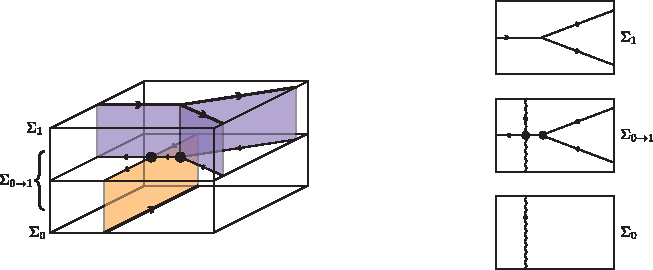
\includegraphics{CellDecomposition.pdf}
\caption{\label{CellDecomposition}
\dave{Will pitchforkize.} \ethan{Actually, I think it might be clearer if you don't. We mention the standardization procedure after we talk about the cell decomposition extension, and I think the figure is easier to look at pre-pitchforkization} 
The decomposition used to construct the shadow world tensor network, shown 
in its pre-standardized, pre-pitchforkization state.
The top layer $\Sigma_1$ is the cell decomposition that we use to construct the Hamiltonian in \eqref{ham}.
The bulk cell decomposition $\Sigma_{0\ra1}$ is found by extending $\Sigma_0$ into 
$\Sigma \times [0,\frac{1}{2}]$, and $\Sigma_{1}$ into $\Sigma \times [\frac{1}{2},1]$ (left figure).
The input cell decomposition $\Sigma_0$ is taken to be in `normal' position with respect to $\Sigma_1$, meaning that when each cell decomposition is extended into the bulk, the two decompositions only intersect transversely along edges. 
On the right, we have shown two dimensional representations of small patches of the cell decomposition. 
In the two dimensional pictures we will denote the cells stemming from $\Sigma_0$ by squiggly lines.
Notice that the orientation of all lines on $\Sigma_{0 \ra1}$ have been reversed relative to $\Sigma_0$ and $\Sigma_1$. 
}
\end{center}
\end{figure}

In order to evaluate $Z(\Sigma_{0\ra1}; v_0, v_1)$, we need to specify a cell decomposition on $\Sigma_{0\ra 1}$ (although the actual partition function is independent of the particular choice). 
We can take the cell decomposition in the bulk of $\Sigma_{0\ra1}$ to be any cell decomposition that agrees with the cell decomposition of $\Sigma_0$ and $\Sigma_1$ when restricted to $\partial \Sigma_{0\ra1}$.
However, there is a particularly convenient choice, which corresponds to extending the cell decomposition of $\Sigma_0$ into $\Sigma \times [0, 1/2]$, and that of $\Sigma_1$ into $\Sigma \times [1/2, 1]$, see Figure~\ref{CellDecomposition}. 
When we do this extension, every $k$-cell in $\Sigma_0$ and $\Sigma_1$ is extended into a $(k+1)$-cell in the bulk 
of $\Sigma_{0\ra1}$ (the $(k+1)$-cells are the `shadows' of the $k$-cells, and hence the bulk constitutes the `shadow world'\dave{never made that connection before, is that why they called it the shadow world?}). 
It is convenient to take the two cell decompositions on $\Sigma_0$ and $\Sigma_1$ to be in `normal' position,
meaning that the extension of $\Sigma_0$ into the bulk only intersects the extension of $\Sigma_1$ transversely along edges, again see Figure~\ref{CellDecomposition}.


We now specify the amplitude $Z(\Sigma_{0\ra 1}; v_0, v_1) $ in \eqref{GroundState}.
The amplitude is determined using the state sum procedure developed previously, and as such we will be brief in what follows. 
The labels of the 2-cells that extend from $\Sigma_0$ and $\Sigma_1$ are determined by $v_0$ and 
$v_1$, since they are the shadows of 1-cells in $\Sigma_0$ and $\Sigma_1$. 
The 2-cell labels living at $\Sigma \times \{ 1/2 \}$ are not fixed as input data however, and need to be 
summed over.

As described previously, to construct the tensors for a given 0-cell $v$ in $\Sigma \times \{1/2\}$, we insert a small $S^2$ around 
$v$ and examine the intersections of neighboring 2-cells with the $S^2$. These intersections 
are marked on the $S^2$ as edges, and weights for the tensor $T_v$ are formed by evaluating 
the picture formed by these edges. 

\begin{figure}
\begin{center}
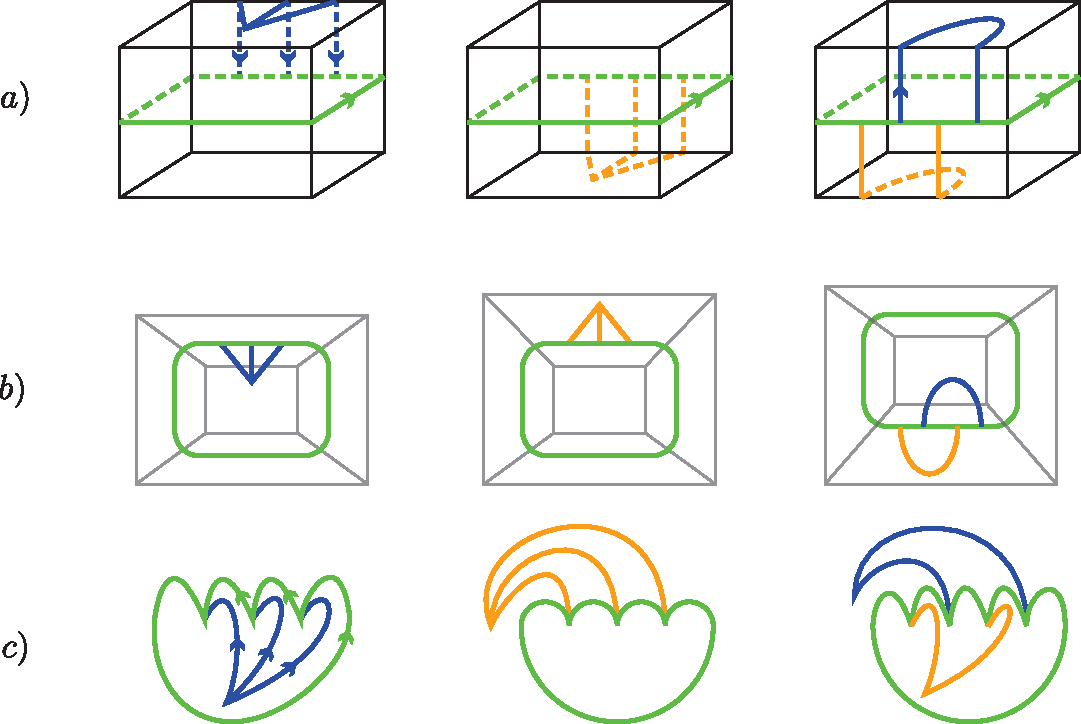
\includegraphics[scale=0.6]{StandardizedSlabTensors.pdf}
\caption{\label{StandardizedSlabTensors}
In row a) we show the three kinds of possible 0-cell tensors that could appear in the tensor contraction when 
computing the partition function $Z(\Sigma;v_0,v_1)$. The cube is drawn so that the 0-cell is located in the cube center. 
Blue (orange) lines represent intersections of 2-cells in the extension of the cell decomposition $\Sigma_1$ ($\Sigma_0$) with the cube, and 
green lines represent intersections of 2-cells in $\Sigma \times \{1/2\}$ with the cube. 
In row b) we show the first step for one possible standardization procedure, where the diagrams 
have been drawn projected into two dimensions. 
In row c) we finish the standardization of the diagrams by making each trivalent vertex a pitchfork. The appropriate 0-cell 
tensors are found by evaluation of these diagrams. 
}
\end{center}
\end{figure}

By looking at Figure~\ref{CellDecomposition}, we see that there are only three kinds of 0-cells that show up in 
$\Sigma \times \{1/2\}$: those that are formed at the x-shaped intersection of a 1-cell in the extension of $
\Sigma_0$ with a 1-cell in the extension of $\Sigma_1$, those where a 0-cell in the extension of $\Sigma_0$ 
meets the interior of a 2-cell in 
the extension of $\Sigma_1$, and vice versa. These possibilities lead to three different types of 0-cell tensors that need to be evaluated. 
These three possibilities are illustrated in the top row $a)$ of Figure \ref{StandardizedSlabTensors}, where we have drawn a cube surrounding the 0-cell instead of an $S^2$.
In the figure, the blue (orange) lines denote 
the intersections of 2-cells in $\Sigma \times (1/2,1]$ (in $\Sigma \times [0,1/2)$) with the cube, 
and the green lines denote the intersection of 2-cells in $\Sigma \times \{1/2\}$ with the cube. 
The orientation of the lines drawn in these figures is fixed by the orientations of each of the 2-cells, 
which are determined with the aid of the orientation of $\Sigma$. 
In order to facilitate computations, we will need to standardize these diagrams according to the 
usual `pitchforkization' procedure employed in the previous sections. 
To do the standardization, we first project the diagrams into the plane (shown in the second row 
of Figure \ref{StandardizedSlabTensors}), and then deform each of the trivalent vertices 
to pitchforks. The final standardized diagrams are displayed in the third row of Figure \ref{StandardizedSlabTensors}.

The evaluation of these standardized diagrams gives the weight of the 0-cell tensor
in the computation of the partition function. 
Explicitly, for a 0-cell $v$ involving three neighboring 2-cells from the extension of $\Sigma_1$ (left column of row $a)$ in Figure \ref{StandardizedSlabTensors}, we assign the tensor $T_v$ as follows:
\begin{align}
\Tensora \; \ra T_v&= \;  \Tensoraa \cdot \mu_0 \tp s_1 \tp s_2 \tp s_3.
\end{align}
In the diagrams, the green letters $A,B,C$ denote the labels of the 2-cells in $\Sigma \times \{1/2\}$, which will 
be summed over when computing the amplitude $Z(\Sigma_{0\ra1}; v_0, v_1)$. The labels of 
the blue lines are fixed however, and determined by the labels of the 2-cells which are shadows of 1-cells 
in $\Sigma_1$. 

Tensors for the other types of 0-cells in $\Sigma \times \{1/2\}$ are determined similarly. For the type of 
0-cell in the center column of row $a)$ in Figure \ref{StandardizedSlabTensors}, we assign the tensor
\begin{align}
\Tensorc \;\ra T_v &= \; \Tensorcc  \cdot \nu_0 \tp s_1 \tp s_2 \tp s_3, \\
\end{align}
while for the type of 0-cell in the last column we assign the tensor
\begin{align}
\Tensorb \; \ra T_v &= \;  \Tensorbb  \cdot s_0 \tp s_1 \tp s_2 \tp s_3, \\
\end{align}
which corresponds to a string operator. 
In all of these tensors, we are making use of the implicit left-to-right Koszul ordering convention for the 
tensor factors. 


In order to perform the contraction that will compute the partition function, all the 1-cells 
$\Sigma \times \{1/2\}$ need an orientation. Since these 1-cells biject with the 1-cells of $\Sigma_0$ and $\Sigma_1$ (they are all shadows of 1-cells in either $\Sigma_0$ or $\Sigma_1$ from our 
choice of cell decomposition in $\Sigma_{0\ra1}$), we can assign an orientation to each 1-handle in 
$\Sigma \times \{1/2\}$ using the orientation of the 1-cells in $\Sigma_0$ and $\Sigma_1$, which 
are fixed by the states $v_0$ and $v_1$.

We can now compute $Z(\Sigma_{0\ra1}; v_0, v_1)$ 
using the state sum: 
\begin{align} 
Z(\Sigma_{0\ra1}; v_0, v_1) = \sum_{ \mcl_{bulk} } (-1)^{k_{\mcl_{bulk}}} \prod_{f \in [\Sigma \times \{1/2\}]_2} T_f(w_f) 
\prod_{e \in [\Sigma \times \{1/2\}]_1} T_e(w_e) \prod_{v \in [\Sigma \times \{1/2\}]_0} T_v(w_v),
\end{align} 
where we have used $[\Sigma \times \{1/2\}]_k$ to denote the collection of $k$-cells in $\Sigma \times \{1/2\}$ and $\mcl_{bulk}$ 
to denote colorings of the bulk degrees of freedom in $\Sigma_{0\ra1}$ for which $\chi(\omega_{\mcl_{bulk}})\neq 0$. 

